\documentclass[a4paper,12pt,twocolumn]{article}

\usepackage[version=3]{mhchem} % for easily typeset chemistry formulae
\usepackage{amsmath,amsfonts,amsthm}
\usepackage{mathptmx}
\usepackage{xcolor} % for colour
\usepackage{titlesec}
\usepackage{fancyhdr}
\usepackage{geometry}
\usepackage{graphicx}
\usepackage[font=small,labelfont=bf]{caption} % makes all captions bold and small
\usepackage{float} % allows me to force placement of figures

\DeclareCaptionType[fileext=los,placement={!ht}]{scheme} % so that we can have items such as reaction schemes
\newtheorem{thm}{Derivation} % so that we can have items such as derivations

\usepackage[
    backend=biber,
    style=chem-acs,
  ]{biblatex}
\addbibresource{hexsi.bib}


\titleformat{\section}{\color{black}\bfseries\filcenter\uppercase}{}{0em}{}

\date{}

\title{Building Nanostructured Porous Silica Materials Directed by Surfactants} % defines the title
\linespread{1.1}

\geometry{a4paper,
          total=          {210mm,297mm},
          left=            14.5mm,
          right=           14.5mm,
          top=             25mm,
          bottom=          25mm,
          bindingoffset=   0mm}


\newlength{\myoddoffset}
\setlength{\myoddoffset}{\marginparwidth + \marginparsep}
    
\fancyheadoffset[leh,roh]{\marginparsep}
\fancyheadoffset[loh,reh]{\myoddoffset}

\pagestyle{fancy}
\fancyhf{}
\lhead{\small{\textit{\textbf{Building Nanostructured Silica Directed by Surfactants}}}}
\rhead{\small{Wayne Yeo Wei Zhong}}
\rfoot{\thepage}
%\cfoot{CONFIDENTIAL}

\begin{document}

%\author{Wayne Yeo Wei Zhong}
%\date{Today}
%\maketitle

	\section{1. Introduction}
	Silica is of central importance in nanomedicine. The suitability of silica nanoparticles in various in vivo biomedical applications, including drug delivery, encapsulation \cite{slowing2008} and fluorescence imaging \cite{ow2005} has been established in previous work \cite{liberman2014}. This is largely by virtue of its biodegradability, biocompatibility and low toxicity \cite{popplewell1998}. The thermal and mechanical stability of silica, with its low density and high specific surface area, lends itself to numerous applications \cite{xu2006}.
	
The synthesis of colloidal silica, consisting of monodisperse nano- to micrometer sized silica nanoparticles, was first described in 1968 \cite{stober1968} and is now known as the St\"ober process. It is a sol-gel process whereby a silicon alkoxide precursor undergoes hydrolysis with water in an alcohol solution containing ammonia as a catalyst, with the resulting molecules condensing to form larger structures. The process has been intensively researched since its discovery, with recent developments substantiating modified processes which utilize a similar sol-gel approach to the synthesis of silica nanostructures in aqueous solvents at neutral pH for convenient and environmentally sound processing \cite{yang2008}. In addition, simple modifications of the sol-gel approach through composition doping can lead to the incorporation of various ions into the silica nanostructure \cite{pohaku2012} to modify material properties.

Tremendous efforts have been made to develop synthetic strategies which allow researchers to access different nanostructures of silica materials, with templated synthesis being a notably effective technique for the controlled synthesis of nanostructured materials \cite{liu2013}. A pre-existing template, or structure-directing agent (SDA), with desired nanoscale features direct the formation of silica into unique structural forms that are otherwise difficult to obtain without the directing effect of the template. As a result, templated synthesis is capable of fabricating nanomaterials with a wealth of consistent and well-defined structures, morphologies and properties. A pertinent example demonstrating the templated synthesis of a complex and functional silica nanostructure, is the development of dual-porosity hollow silica nanospheres as a vehicle to deliver nonhuman enzyme therapies \cite{ortac2014}. Such morphological precision was attained through templating with existing colloidal polystyrene nanoparticles as templates and nanomasks \cite{trogler2013}. This demonstrates the utility of the synthesis described by Yang and colleagues with appropriate hard colloidal physical templates.

In addition to hard templating strategies, soft template methods ranging from emulsions, micelles or vesicles, to some polymers and biological molecular assemblies have been developed. The principal advantage of soft template synthesis is the capacity to synthesize different materials with various non-traditional morphologies \cite{wan2007}. The fabrication of amorphous hexagonal silica platelets with a template-based biomimetic synthesis, through using polypeptides such as poly-\textsc{l}-lysine (PLL) \cite{tomczak2005,bellomo2006} has been reported. However, the synthesis described by Tomczak and colleagues is dependent upon the unstable secondary structure transition of PLL coils to alpha helices. The failure to undergo a secondary structure transition to adopt a helical conformation would result in the loss of any templating ability. A robust and flexible fabrication approach that allows for the synthesis of a wide variety of nanostructures, over the variation of a broad range of precise reaction conditions has yet to be developed, and remains a key objective for the community.

To achieve the above objective, this study shifts our attention to another class of molecules with a flexible structure-directing ability. Surfactant systems self-assemble to form different aggregate structures at ambient conditions, resulting in a diverse range of isotropic micellar solution and lyotropic liquid crystal phases in aqueous solution. Microstructures in surfactant systems are governed by the interplay of geometrical constraints \cite{israelachvili1976} and electrostatic interactions due to different counterions \cite{kang1993}. In addition, microstructure formation can also be influenced by the addition of salts and other electrolytes \cite{thalberg1991}. The richness of aggregation behaviour indicates that there is much potential in the use of surfactants as structure-directing agents in soft template syntheses. 

Hierarchical mesoporous structures have been reported by templating on soft templates of orderly arranged liquid crystalline surfactant micelles \cite{colfen2007}. One such material is MCM-41 \cite{kresge1992}, which involves a hydrothermal sol-gel reaction templated by a hexagonal \textit{P6m} phase of cetyltrimethylammonium bromide (CTAB) surfactant, yielding a three-dimensional ordered mesoporous silica material with non-intersecting hexagonal channels. 

An interesting candidate as a structure-directing agent for soft template synthesis of silica at ambient conditions is the cationic surfactant, didodecyldimethylammonium phosphate (Fig. 1). The preparation, self-assembly and phase behavior of double-tailed didodecyldimethylammonium (\ce{DDA+}) surfactants have been extensively studied in the literature \cite{warr1988}. The microstructure formation of \ce{DDA+} surfactants have been found to be sensitive to the surfactant concentration and speciation of its hydrolysable counterions \cite{liu2014}. In this research, we chose \ce{DDA+} phosphate systems as a structure-directing agent, primarily because double-tailed surfactants have largely been unexplored and underexploited as soft templates for the synthesis of silica nanostructures. In addition, \ce{DDA+} phosphate has unique prolate micellar phases that are stabilized by a hydrolysable phosphate counterion. This project aims to study the effects on the morphology of silica nanostructures templated by \ce{DDA+} phosphate surfactant when varying reaction conditions such as surfactant concentration and reaction temperature.

	\begin{figure}[h]
		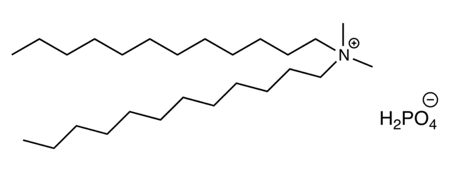
\includegraphics[width=\linewidth]{structure.png}
  		\caption{Molecular structure of \ce{DDAH_2PO_4}, the major species of \ce{DDA+} phosphate present in synthesis}
  		\label{fig:structure}
  	\end{figure}
	 
	 \section{2. Methods}
	 
	 \paragraph{2.1 Materials.} Milli-Q water prepared by a SGwater UltraClear Basic TWF system with a resistivity of 18.2 M$\Omega$ cm was used for all reactions and dilutions in this study. Amberlite IRA-400(OH) resin and orthophosphoric acid (85 wt. \%) were obtained from Sigma-Aldrich. pH measurements were made with a Metrohm 827 pH lab meter. Tetramethoxysilane (TMOS) was used as received from Merck. Methanol was obtained from J. T. Baker. Didodecyldimethylammonium bromide (DDAB, 98\%) was purchased from TCI. 
	 
	 \paragraph{2.2 Preparation of starting materials.} Dilute phosphoric acid was prepared by diluting concentrated orthophosphoric acid with water. DDAB was dissolved to form a colorless solution in a methanol-water solvent. Didodecyldimethylammonium hydroxide (DDAOH) was prepared by substituting bromide ions with hydroxide ions from DDAB using the Amberlite ion exchange resin for 24 h. The successful conversion of the counterion from bromide to hydroxide was verified using pH measurements to confirm that the DDAOH is highly alkaline (pH ≈ 12.8). Methanol from DDAOH was removed through rotary evaporation, which yielded a clear, viscous solution of aqueous DDAOH. The final \ce{DDAH_2PO_4} was then prepared by titrating dilute phosphoric acid into DDAOH solution to an appropriate equivalence of pH 7.02, which indicates that the hydroxide ions are successfully neutralized to a buffer system of phosphate species (\ce{H_2PO4-}/\ce{HPO_4^2-}). The clear, viscous solution of aqueous \ce{DDAH_2PO_4} was then freeze-dried and isolated as a fine white powder. In this study, we denote the phosphate surfactant used in synthesis as \ce{DDAH_2PO_4}, because the predominant counteranion was later determined to be \ce{H_2PO4-}, though it coexists with a minor fraction of \ce{HPO_4^2-}.
	 
	 \paragraph{2.3 Synthesis of templated silica nanostructures.} 5 wt. \% stock \ce{DDAH_2PO_4} solution was prepared by dissolving the previously prepared anhydrous powdered \ce{DDAH_2PO_4} in water, which was then equilibrated under mixing for 48 h. Different required concentrations were then drawn from sub-dilutions of different batches of the stock solution. 1 mL of a desired concentration of surfactant solution was equilibrated in a water bath at the desired temperature for 30 minutes. A silica alkoxide source, in our case, tetramethoxysilane (TMOS) was added into the above surfactant solution in one portion. The reaction was conducted on a vortex agitator on a high speed, which provides rapid mixing of reactants. The reaction mixture was then returned into the water bath and retrieved after 24 h. The silica nanostructures were separated from the supernatant by centrifugation as a pellet, and resuspended in deionised water for further characterisation.
	 
	 \paragraph{2.4 Design of the experimental matrix.} The two reaction variables which we determined that are likely to produce a wide range of silica morphologies are the surfactant concentration and solution temperature, as the phase behaviour of similar \ce{DDA+} surfactant systems are known to be responsive to these variables \cite{kang1993}. As such, a range of concentrations and temperatures have been generated from what is feasible, afforded by the viscosity of the solution to ensure homogeneous mixing. We conducted the above sol-gel synthesis experiments at temperatures ranging from 0, 4, 8, 12, 16 and 20 $^\circ$C and concentrations from 0.5, 1.0, 2.0, 3.0 and 5.0 wt. \% to obtain a matrix of silica nanostructures yielded at each reaction condition.
	 
	 \paragraph{2.5 Scanning electron microscopy.} SEM images were taken using a Jeol JSM-7600F Schottky Field Emission Scanning Electron Microscope by Dr. Su Hui Lim at the Institute of Materials Research and Engineering, A*STAR. Samples were sputter-coated with gold or platinum before microscopy.
	 
	 \section{3. Results and discussion}
	 
	 \paragraph{3.1 Preparation of the \ce{DDA+} phosphate structure directing agent.} \ce{DDAH_2PO_4} was prepared from commercially available DDAB as in Scheme 1. DDAOH was titrated against phosphoric acid, with the resulting pH tracked with a pH meter.
	 
	 \begin{scheme}
	 	\centering
		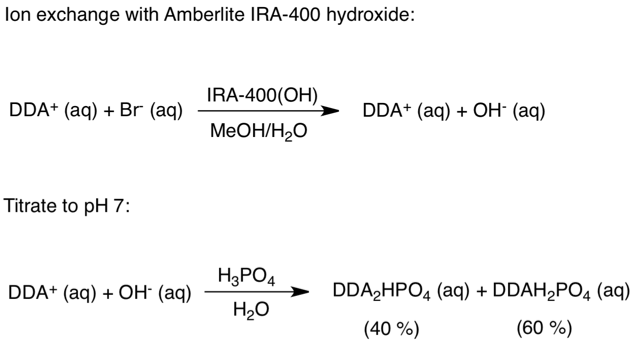
\includegraphics[width=1.05\columnwidth]{surfscheme.png}
  		\caption{Preparation of \ce{DDA+} phosphate from DDAB through an ion exchange and titration.}
  	 \end{scheme}
  	
  	A typical triphasic titration curve was obtained from the titration, shown in Fig. 2. 
  	
  	\begin{figure}[b!]
		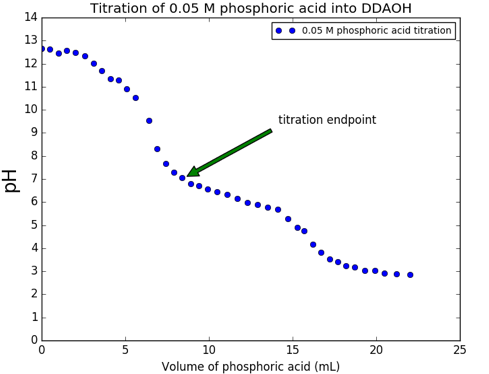
\includegraphics[width=\linewidth]{titration.png}
  		\caption{Triphasic titration curve of phosphoric acid into DDAOH, with the titration endpoint of pH 7.02 indicated by the arrow.}
  	\end{figure}
  	
  	For the purpose of the following synthesis steps, an endpoint of pH 7 was chosen for the titration. During the titration, numerous observable changes to the titre were seen. At pH 13, the titre turned cloudy, with bubbles forming at the surface of the titre. At pH 11.6, the titre adopted the appearance of a milky emulsion. From pH 10.9 onwards, the titre remains a clear, viscous solution until the experimental endpoint of pH 7.02. The visual observations made during the titration of phosphoric acid into DDAOH, as described above, is likely to correspond to the presence of lamellar or vesicle structures in \ce{DDAH_2PO_4} systems with a high fractional composition of \ce{PO_4^3-} counterions \cite{liu2014}. 
  	
  	
  	\ce{DDAH_2PO_4} was determined to be the major surfactant species present, making up 60.6\% of all surfactant species in solution. A minor species of \ce{DDA_2HPO_4} made up the remaining 39.4\%. This is because hydrolysis leads to a distribution of different phosphate counterion species in solution (\ce{H_2PO_4^-}, \ce{HPO_4^2-}, \ce{PO_4^3-}) which can be expressed as a function of solution pH. This is done by firstly considering the $K_a$ expressions for the three deprotonations of phosphoric acid, and expressing the initial concentration of phosphoric acid as the sum of the concentration of all species. 
  	
  	This can be solved as a system of four equations, with the species fractions being expressed as a function of the hydronium ion concentration (see Derivation 1 in the Supplementary Information section). The graph showing the fractional speciation of the phosphoric acid system as a function of pH is displayed as Fig. S1. The fractions of \ce{H_2PO_4^-} and \ce{HPO_4^2-} at the titration endpoint are indicated in the plot.
  	
  	\paragraph{3.2 Synthesis of surfactant-templated silica nanostructures.} Silica templated by the \ce{DDAH_2PO_4} system was synthesised according to Scheme 2, and the methods described in Section 2.3. In the sol-gel synthesis, TMOS is hydrolysed in aqueous solution to give silicic acid, which acts as a precursor for the polycondensation reaction at the nucleation point. The initial chemistry of the process is detailed below \cite{yang2008}. 
  	
  	\begin{figure}[!h]
		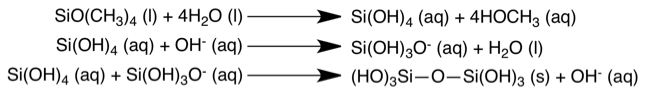
\includegraphics[width=\linewidth]{mechanism.png}
  	\end{figure}
  	
  	  	\begin{figure*}[t!]
  	\centering
		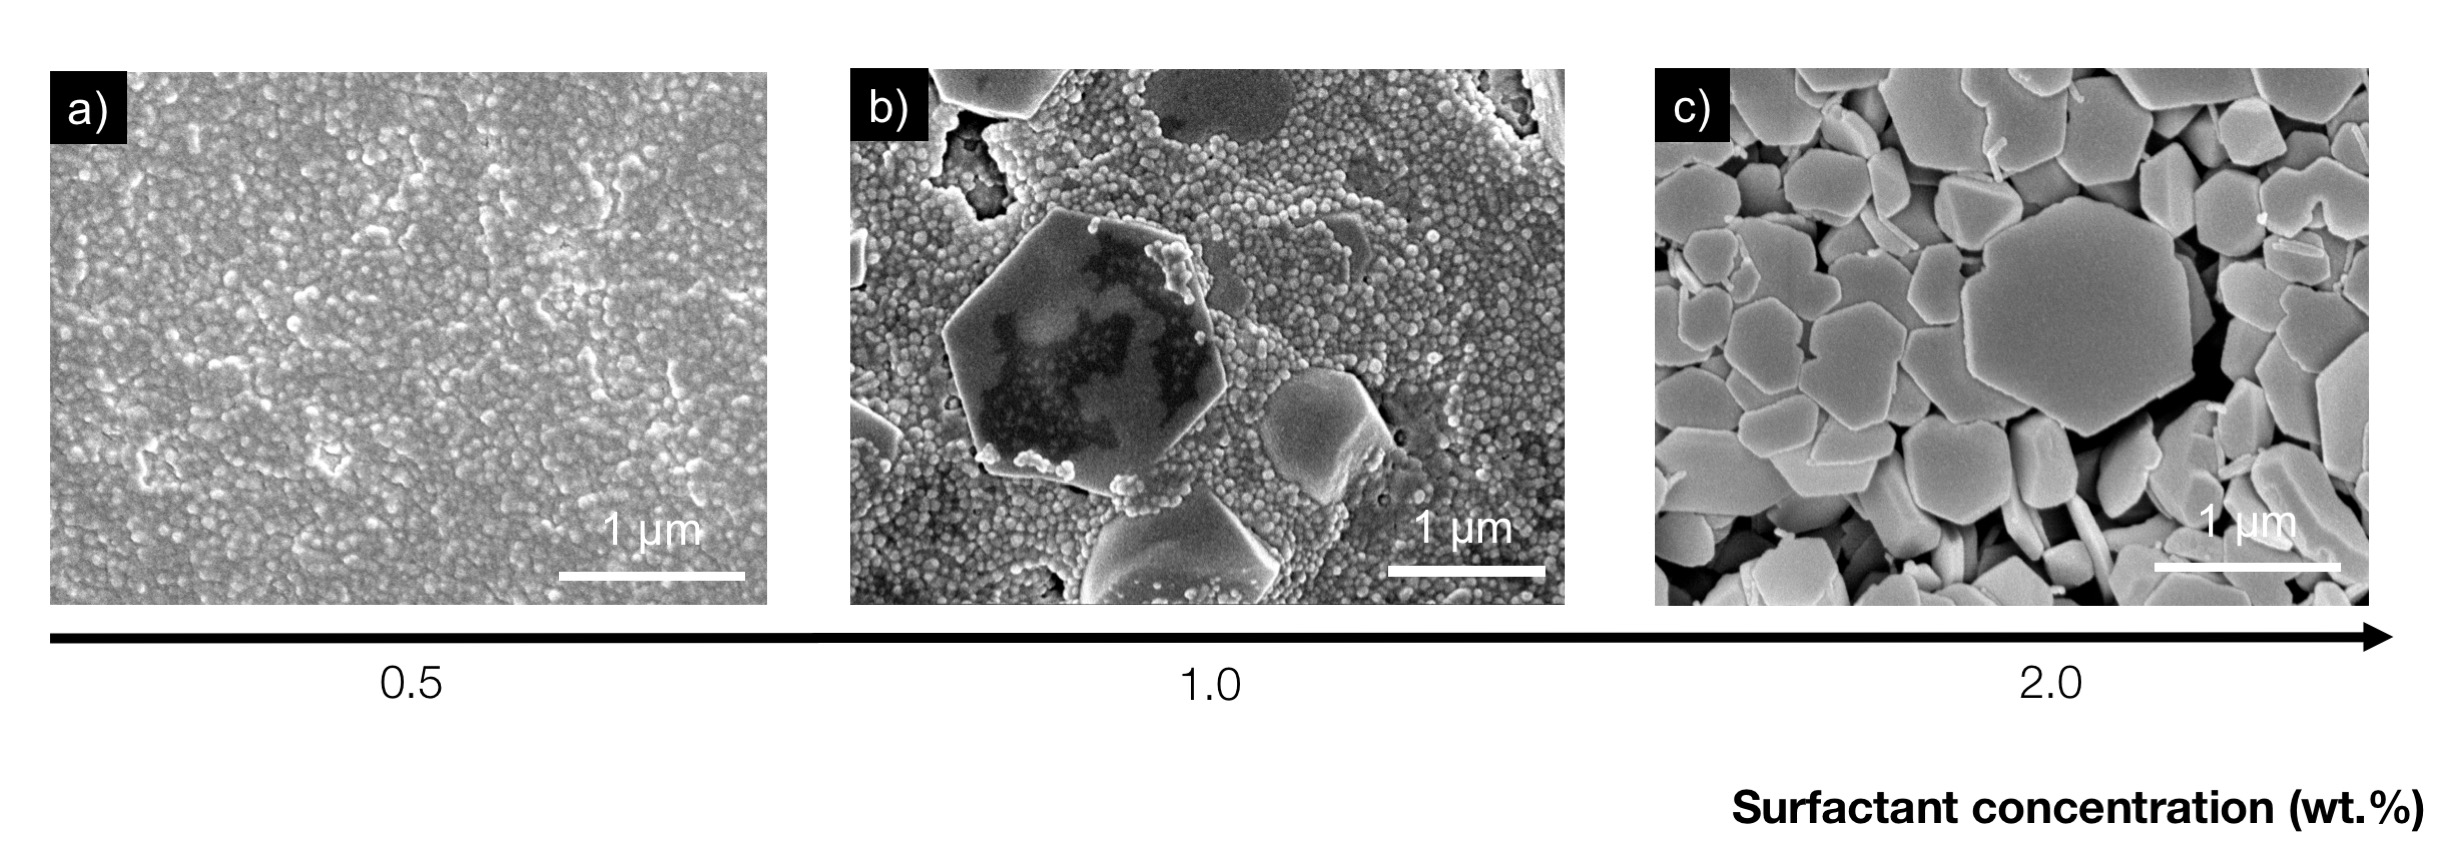
\includegraphics[width=\textwidth]{0deg.jpg}
 		\caption{SEM micrographs of silica structures synthesised at 0 $^\circ$C. (a) 0.5 wt. \%, (b) 1.0 wt. \% and (c) 2.0 wt. \%.}
 	\end{figure*}  
  	The hydrolysis of TMOS is an acid-catalysed reaction, whereas the formation of silicate species and further polymerisation are base-catalysed. We predict that the precipitation reaction can potentially be controlled through preferential precipitation at the high positive charge density at the surface of self-assembled structures of cationic surfactant. This leads to a high concentration of silicate species at the positively charged surfactant headgroup interface, resulting in favourable silicate polymerisation at the surfactant-silicate interface \cite{monnier1993}. The mechanism of the templating employed in this synthesis is still a topic of much debate by the community, but there is a general consensus that the occurrence of direct geometrical templating is improbable \cite{colfen2007}. Instead of geometrical templating, we propose that the electrostatic interactions between cationic headgroups and counterions of the \ce{DDA_2HPO_4} surfactant are postulated to play a significant role in the control of silica formation. It is unknown exactly how the introduction of silica precursors, and the anionic species formed during silification would affect the template’s phase behaviour, and through interacting electrostatically with the template.
  	
  		\begin{scheme}[t!]
	 	\centering
		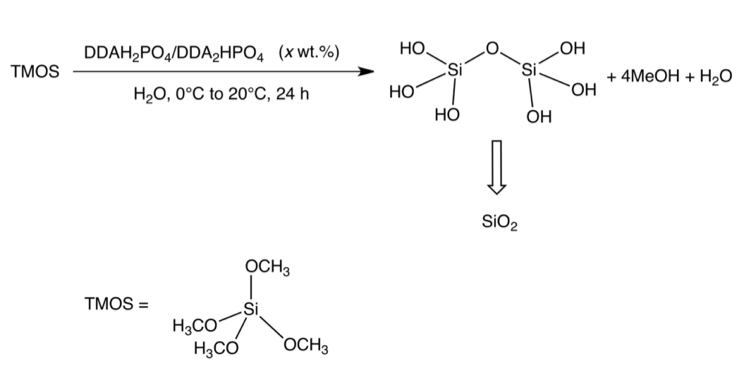
\includegraphics[width=1.05\columnwidth]{silicascheme.png}
  		\caption{Templated sol-gel synthesis of silica, in an aqueous solution at ambient conditions.}
  	\end{scheme}
  	
	
  	
  	\paragraph{3.3 Silica morphologies at 0 $^\circ$C.} The first set of silica was synthesised as described in Scheme 2 at 0 $^\circ$C. SEM was performed to determine its structure and morphology, as shown in Fig. 3. The images reveal that the resulting nanostructures are largely discrete particles and do not form a continuous network.
  	
  	As seen in Fig. 3a, the synthesis at a surfactant concentration of 0.5 wt. \% yielded small silica nanobeads. With an increase in surfactant concentration to 1.0 wt. \%, a mixture of morphologies can be observed (Fig. 3b), indicating an intermediate phase within a transition of morphology. Beads of silica can be found alongside larger hexagonal plates. At 2.0 wt. \%, we observe that the nanobeads are nowhere to be found, with only polygonal plates remaining (Fig. 3c). The gradual transition of morphology from beads to plates demonstrates that we can alter the morphologies of silica nanostructures by varying the concentration of surfactant in solution. As these results were reproducible and corroborated with previous work done within the group \cite{yong2017}, we began the construction of the synthesis matrix.
  	
  	\begin{figure*}[h!]
  	\noindent%
	\begin{minipage}{\linewidth}% to keep image and caption on one page
		\makebox[\linewidth]{%        to center the image
  		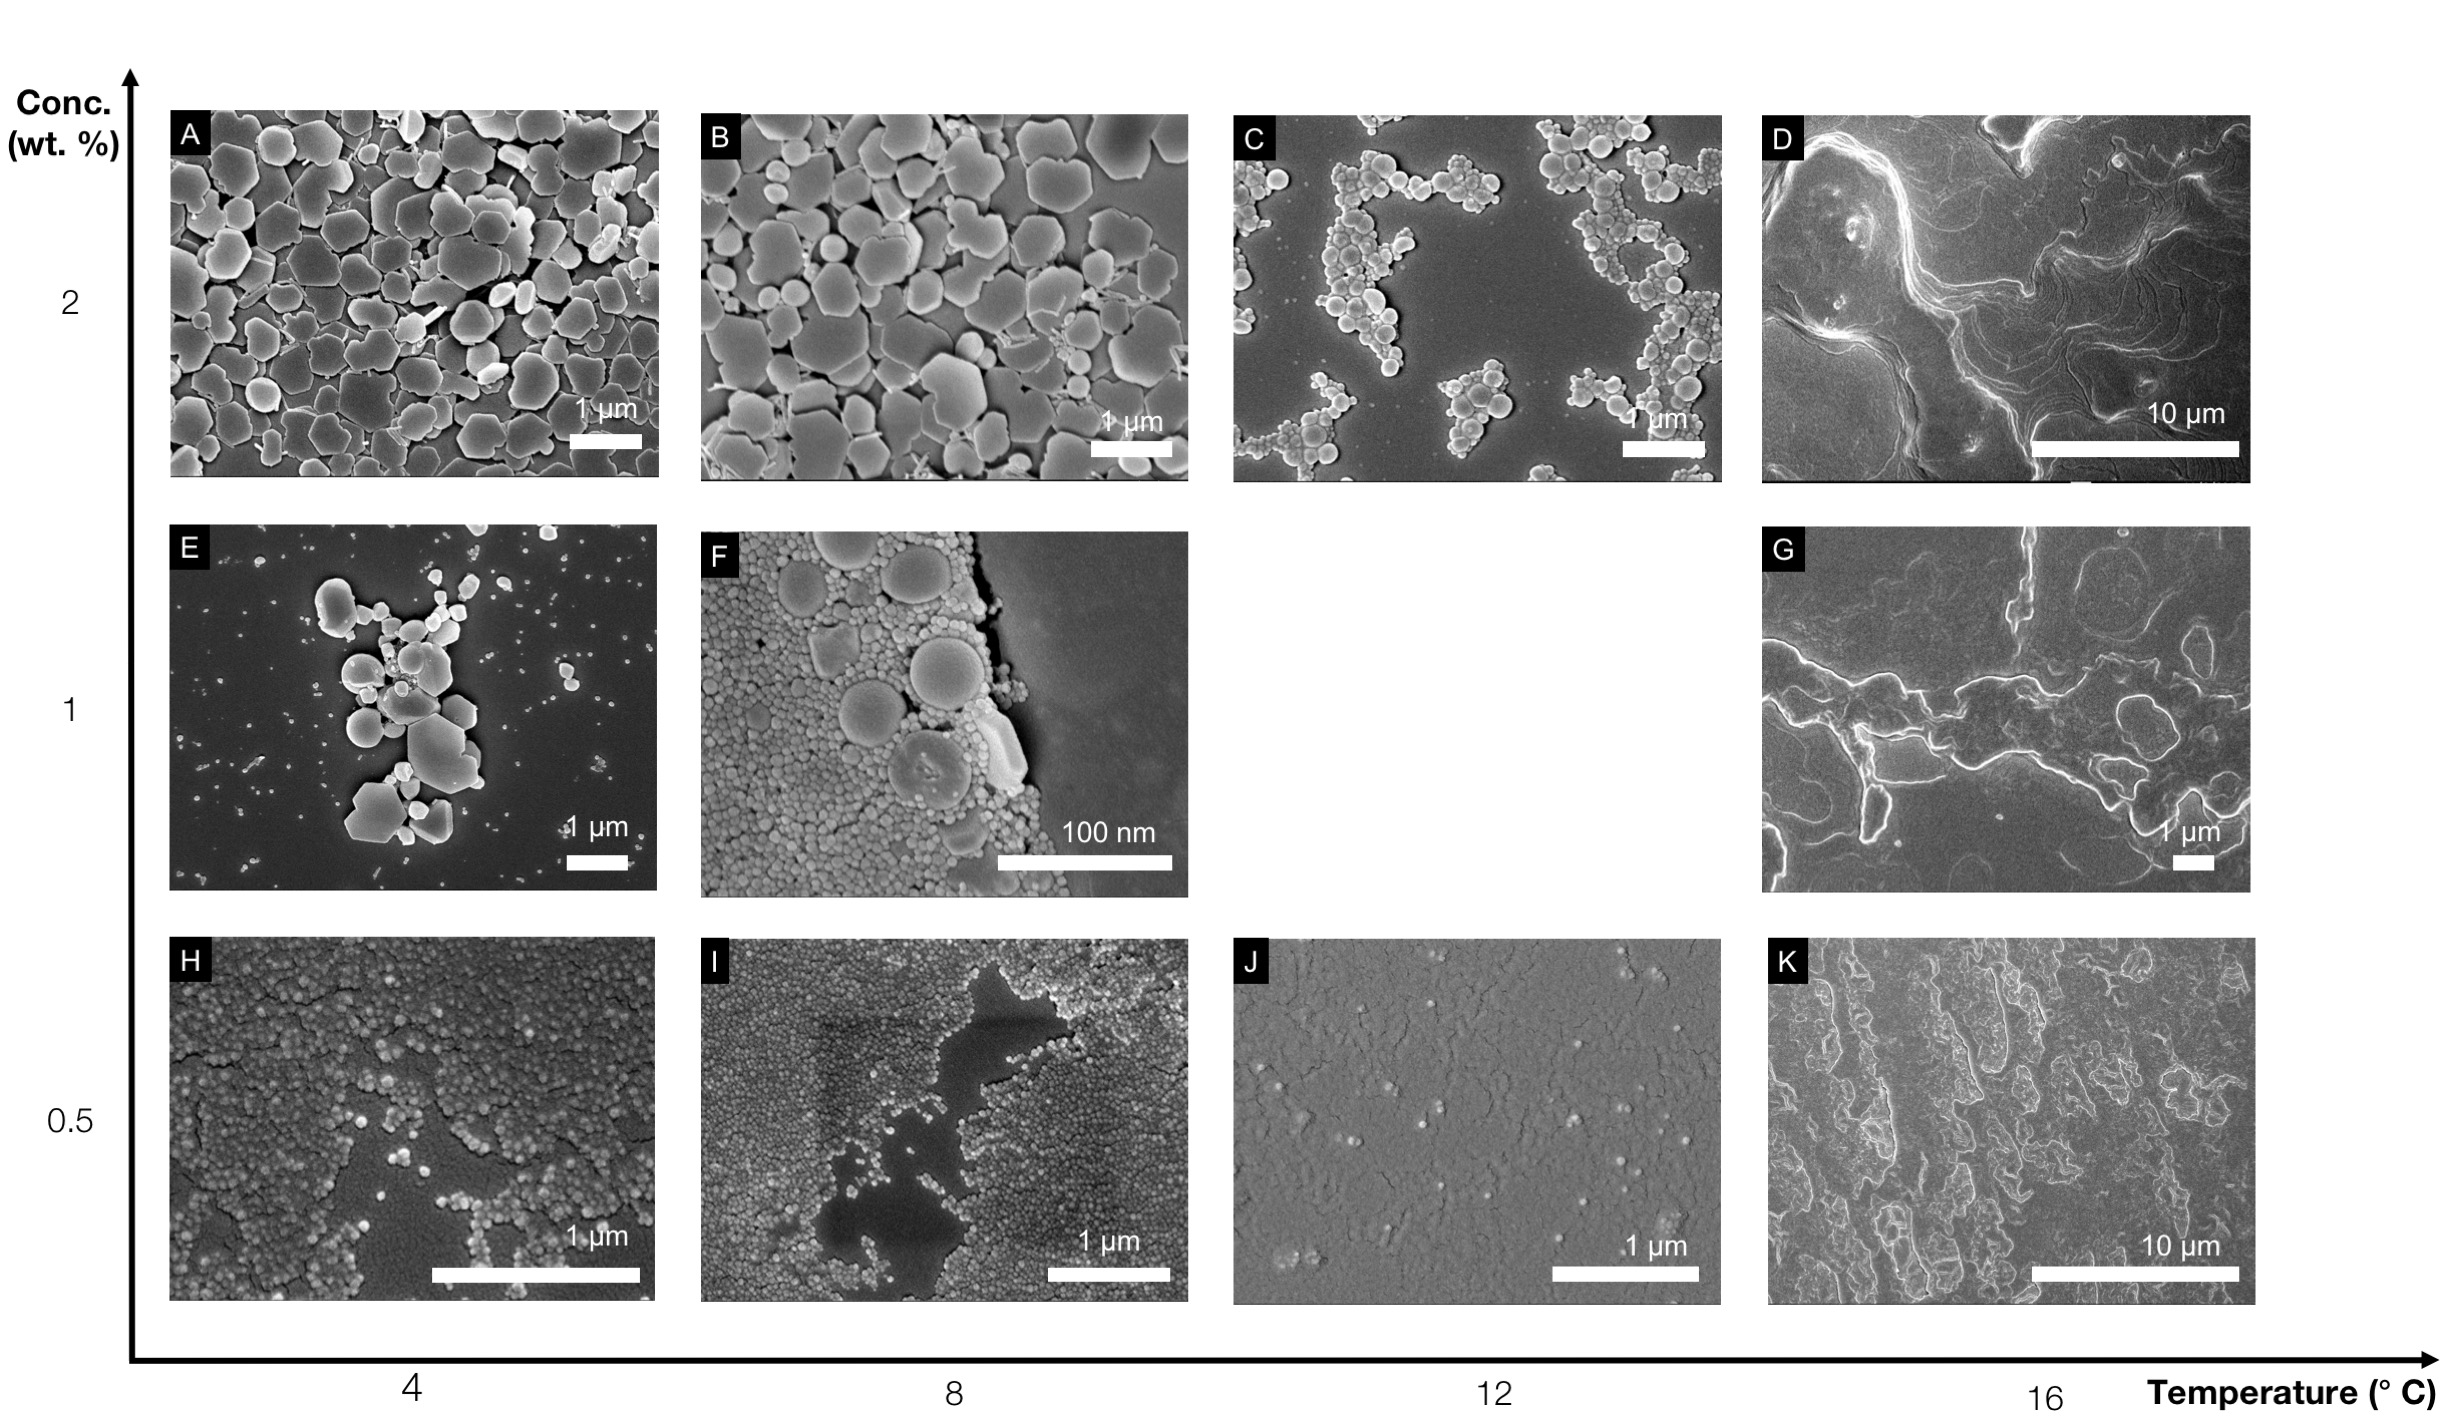
\includegraphics[keepaspectratio=true,width=\linewidth]{lowcon.jpg}}
		\captionof{figure}{(A -- K) Electron micrographs of silica structures made with the surfactant template at various temperatures in a low concentration range (0.5 -- 2.0 wt. \%).} %      only if needed  
	\end{minipage}
	\end{figure*}
  	
  	\paragraph{3.4 Silica morphologies as a function of concentration and temperature.} We then proceeded to conduct the same synthesis displayed in Scheme 2 under the range of reaction parameters (4 -- 20 $^\circ$C and 0.5 -- 5.0 wt. \%) determined in Section 2.3. The morphological and structural properties of the nanostructures at low concentrations are presented in Figure 4, and structures resulting from being templated at high surfactant concentrations are presented in Figure 5.
  	
  %	\begin{figure*}[h!]
 % 	\centering
	%	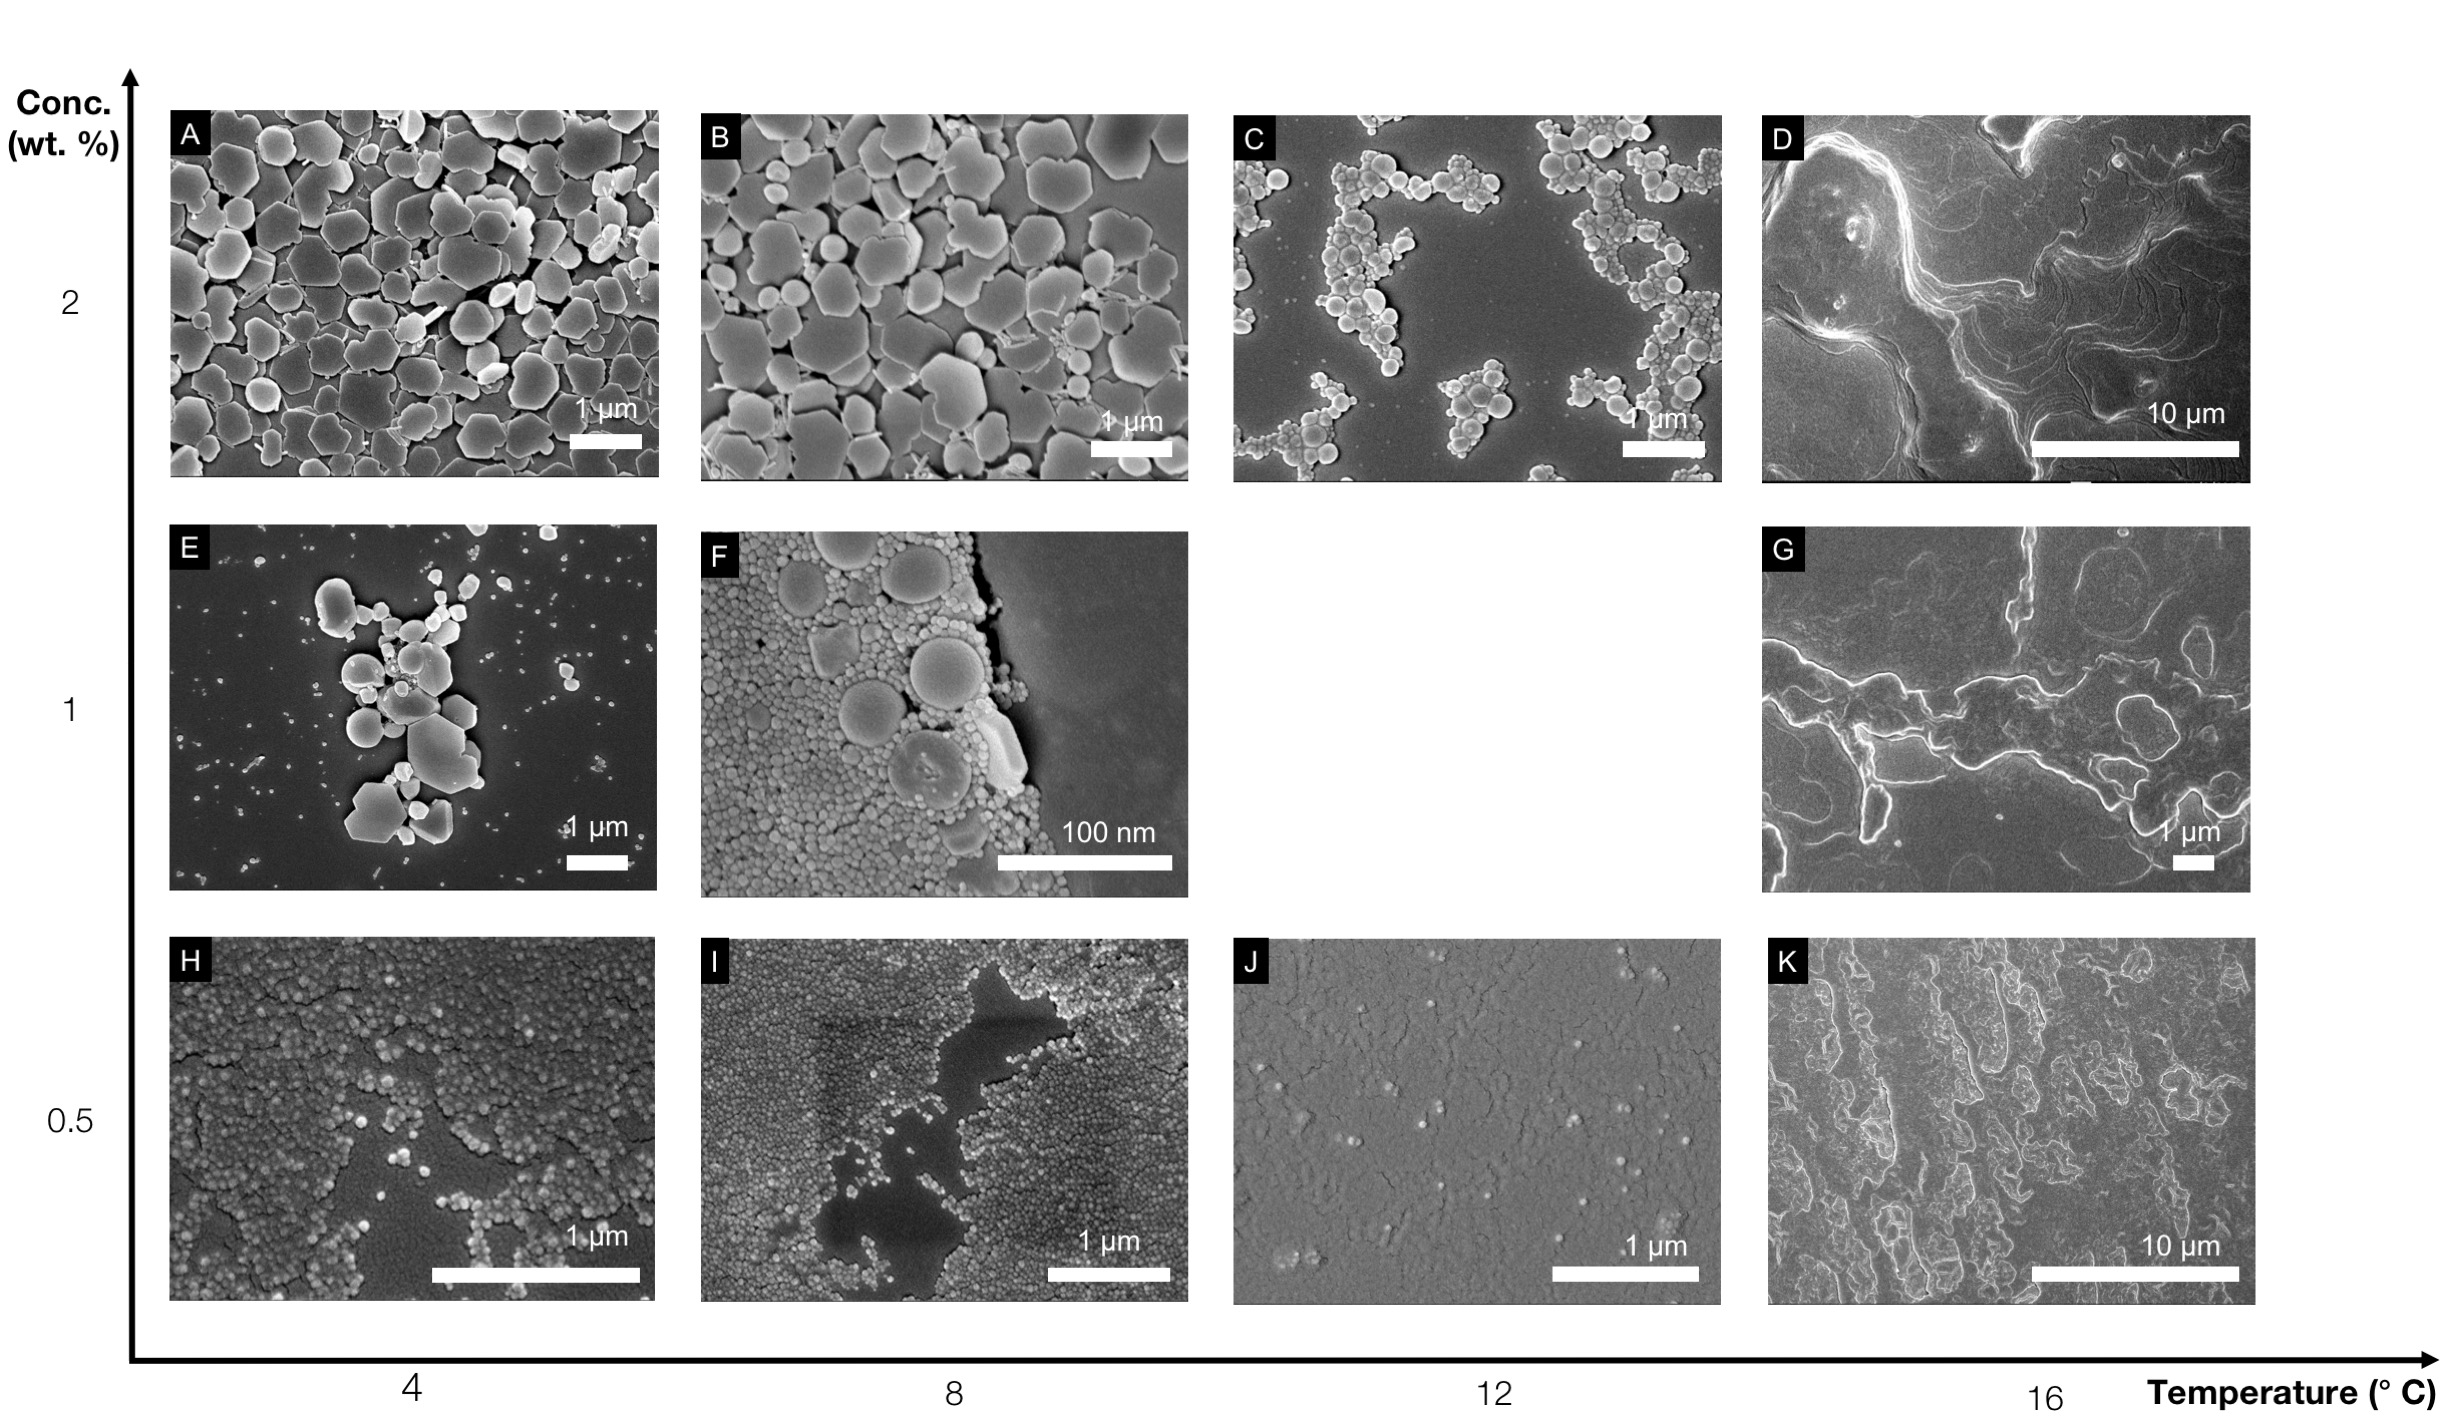
\includegraphics[width=\linewidth]{lowcon.jpg}
  	%	\caption{(A–K) Electron micrographs of silica structures made with the surfactant template at various temperatures in a low concentration range (0.5 – 2.0 wt. \%). }
  %	\end{figure*}
	
  	
  	In Fig. 4, we observe that as concentration is increased from 0.5 wt. \% to 2 wt. \%, there is a general trend that the dimensions of the particles formed increases alongside a shift in morphology, from small nanobeads (Fig. 4H) to larger polygonal plates (Fig. 4A, 4B), with intermediate phases found at a concentration of 1.0 wt. \% (Fig. 4E, 4F). 

  	As the reaction temperature is increased at low concentrations, we observed a loss in templating ability by the surfactant. The pellet of silica that could be retrieved from the supernatant and re-suspended in water became vanishingly small, and the wavy streaks (Fig. 4D, 4G, 4K) in the micrograph resemble colloidal silica or traces of surfactant residue unable to be removed by centrifugation.
  	
  	In Fig. 5, we observe that when the surfactant concentration is increased further at low temperatures, a second transition in morphology from hexagonal plates (Fig. 5E) to concave toroidal structures (Fig. 5A) is observed. These concave structures are approximately 0.5 times smaller than the hexagonal plates that were produced at lower concentrations. It has been previously reported that silica condensation causes the charge density across the silicate network to decrease, causing an increase of the effective headgroup area of the surfactant. As a result, it is more favourable to form surfactant microstructures with high surface curvatures \cite{che2005,israelachvili1976}. We postulate that an increase in surfactant concentration will provide a greater headgroup charge density as the driving force for the transformation from plates to concave structures in a similar fashion.
  	
  	\begin{figure*}[h!]
  	\noindent%
	\begin{minipage}{\linewidth}% to keep image and caption on one page
		\makebox[\linewidth]{%        to center the image
  		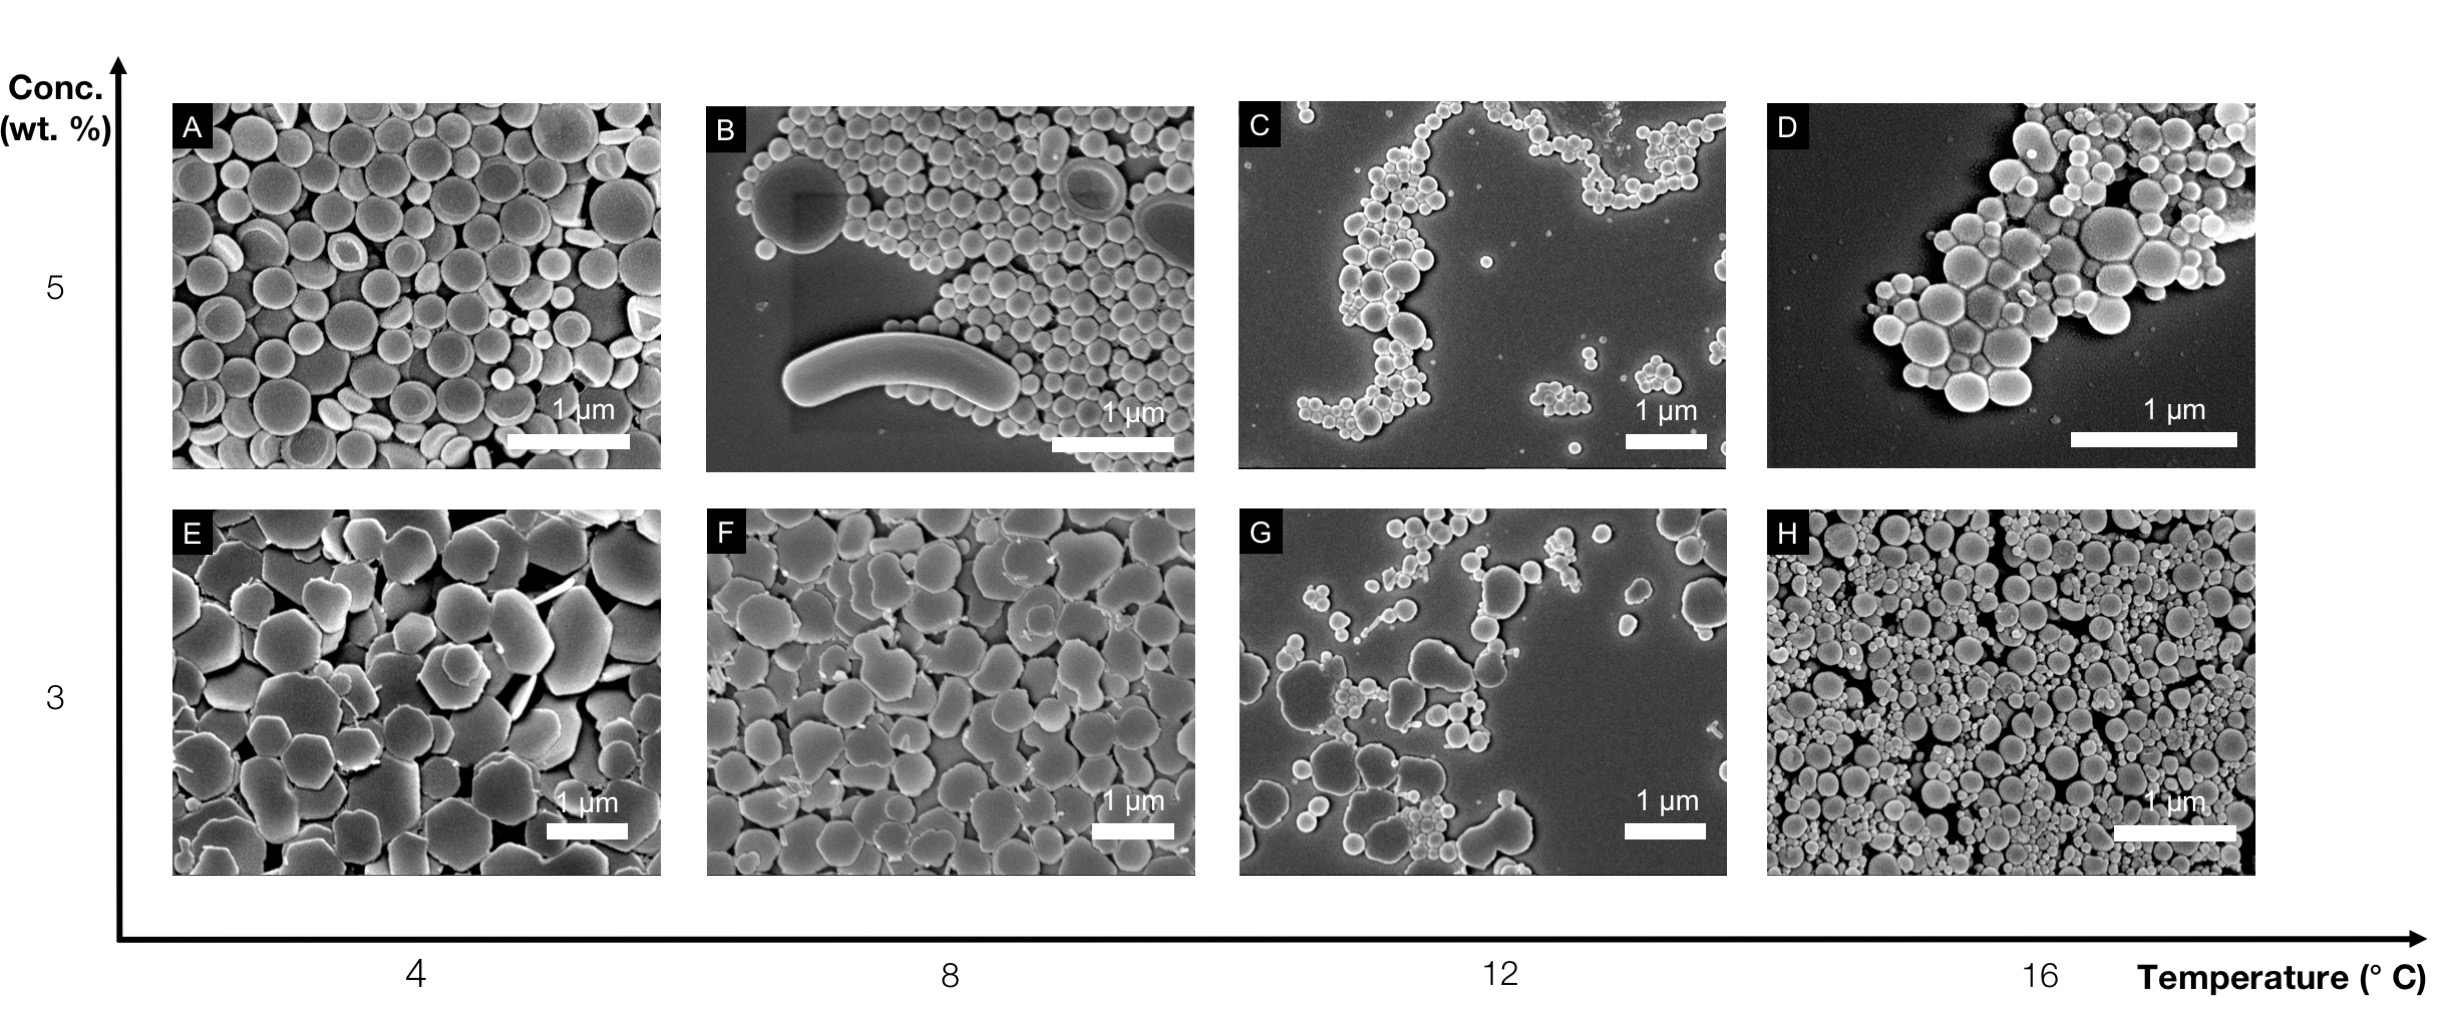
\includegraphics[keepaspectratio=true,width=\linewidth]{highcon.jpg}}
		\captionof{figure}{(A -- H) Electron micrographs of silica structures made with the surfactant template at various temperatures in a high concentration range (3.0 -- 5.0 wt. \%)} %      only if needed  
	\end{minipage}
	\end{figure*}	
  	
 % 	\begin{figure*}[h!]
  %	\centering
	%	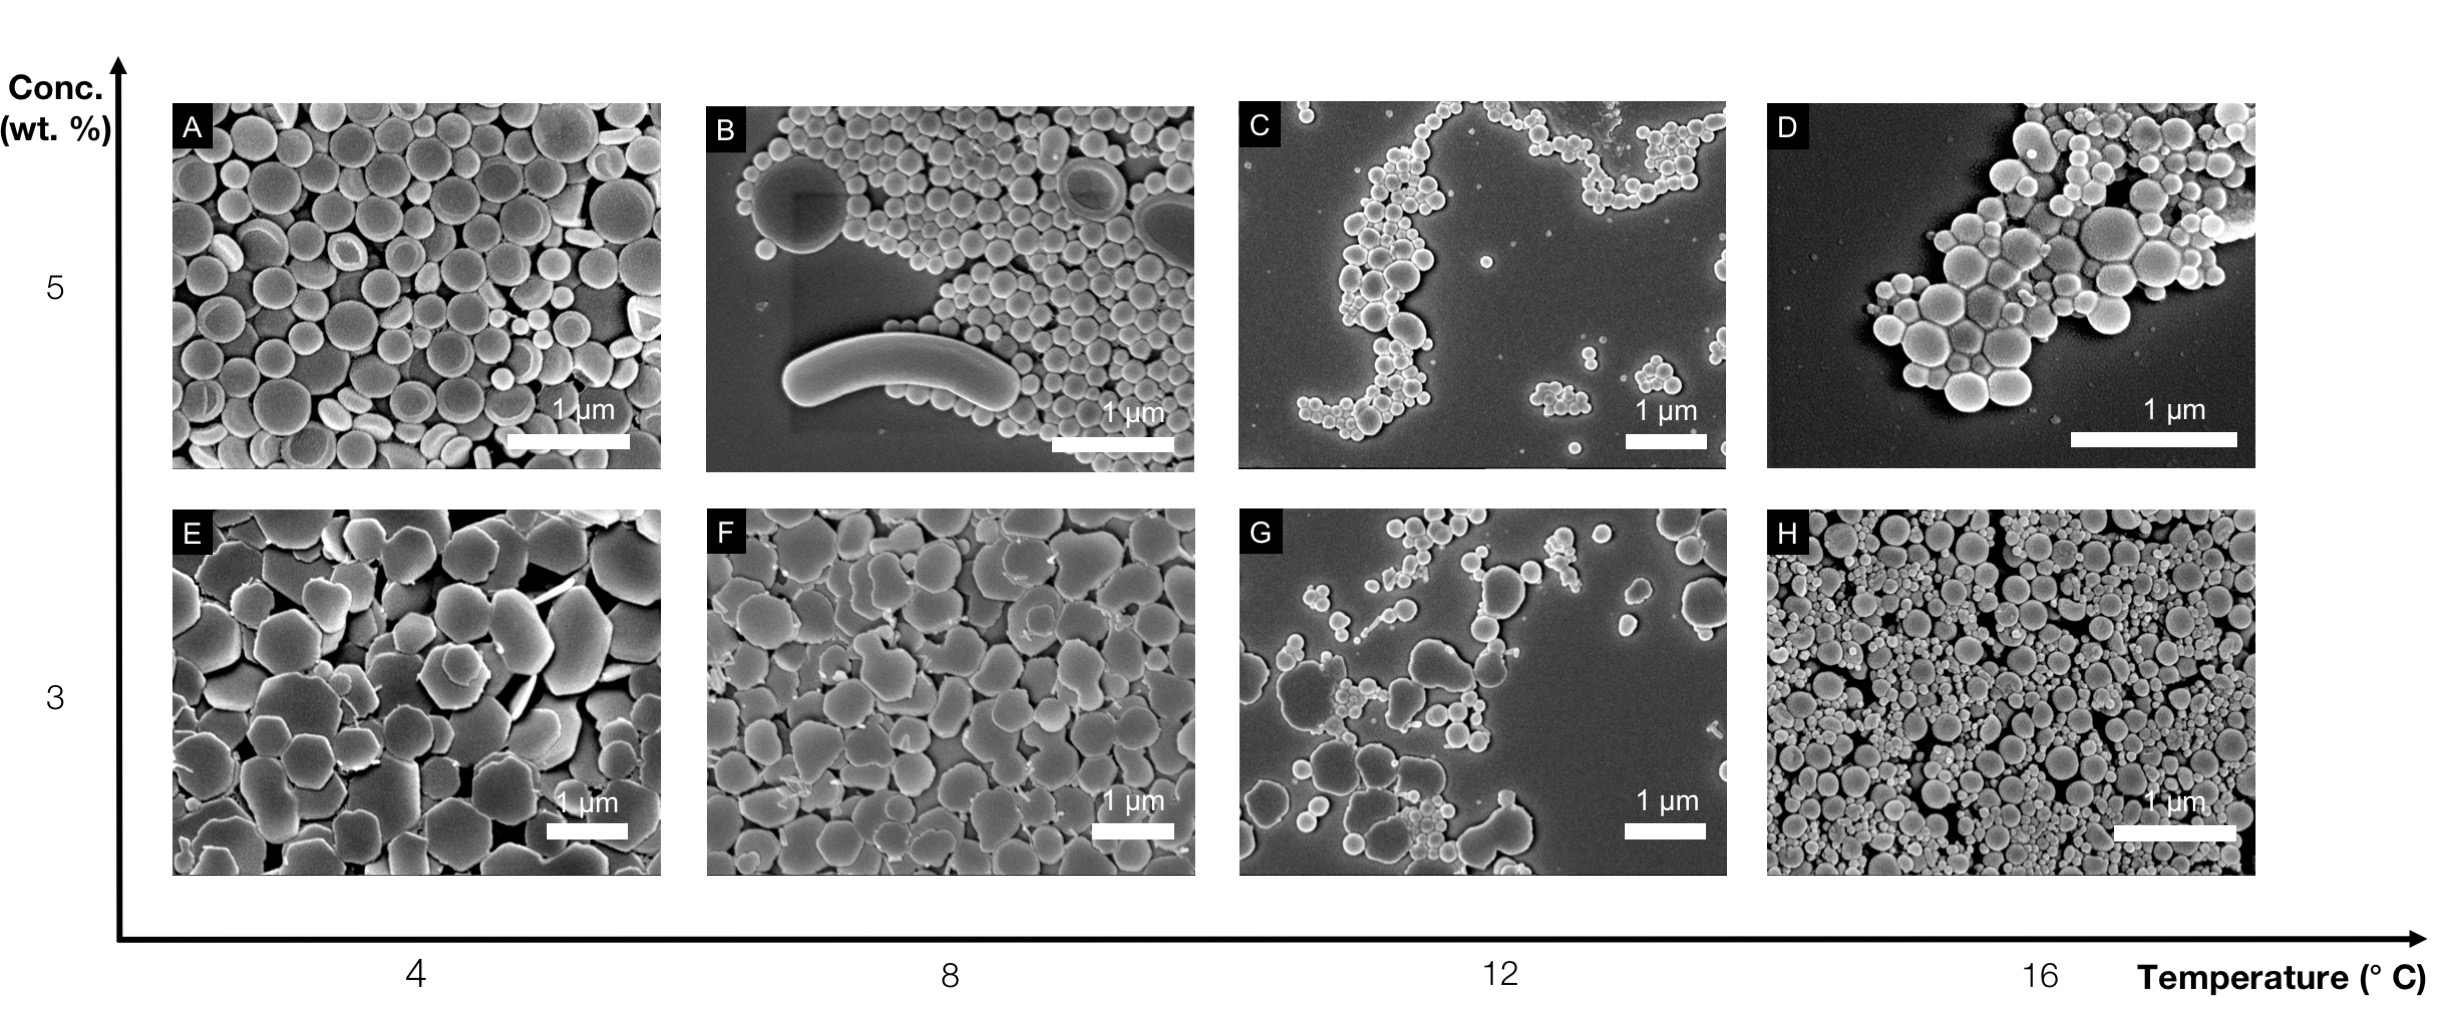
\includegraphics[width=\linewidth]{highcon.jpg}
  %		\caption{(A-H) Electron micrographs of silica structures made with the surfactant template at various temperatures in a high concentration range (3.0 – 5.0 wt. \%)}
  %	\end{figure*}
  	
  	With an increase in temperature, the reactions at high surfactant concentrations produced a range of intermediate morphologies ranging from spheroids, to large toroidal and larger nanorod structures (Fig. 5B), this occurs before the transition into spheroids. We postulate that these structures are yielded by the templating behavior of the surfactant, as they have concave dimensions that are a characteristic feature observed throughout the syntheses at high surfactant concentrations. The wide range of structures can be attributed to a phase transition of the surfactant, forming intermediate structures that the silica templates upon. At high concentrations and temperatures, we see gradual shifts toward more consistent morphologies and size distributions. In this region, we see two main morphologies, nanobeads and larger spheroids, of which some are concave (Fig. 5D, 5H).
  	
  	A number of trends identified from the data collected are summarized in Figure 6. At low temperatures, an increase in surfactant concentration will result in clearly defined morphological transitions from nanobeads, to polygonal plates and concave toroidal particles. Across the range of concentrations that have been investigated in this study, an increase in temperature results in a gradual loss in templating ability by the surfactant, yielding colloidal silica at low surfactant concentrations and spheroidal nanoparticles at high surfactant concentrations.
	 
	 \section{4. Conclusions and future work}
	 
	 In summary, we have shown that the sol-gel method and the surfactant templating approach with \ce{DDAH_2PO_4} as the structure directing agent can be developed into a promising platform for producing a diverse range of functional nanostructures, with varying morphological, architectural and dimensional properties. We have shown the ability to access different morphologies and dimensions of silica nanostructure, such as hexagonal plates and concave toroidal particles with a variation in concentration of the \ce{DDAH_2PO_4} surfactant. Furthermore, an increase in the solution temperature results in a decrease in the structure directing ability of the surfactant, yielding interesting intermediate morphologies. This research has demonstrated that varying easily accessible reaction parameters, such as solution temperature and surfactant concentration, can allow researchers to modulate the structure of silica produced from the same surfactant-templated synthesis, displaying consistent trends in morphology. 
	 
	 	\begin{figure}[!b]
  	 	\centering
		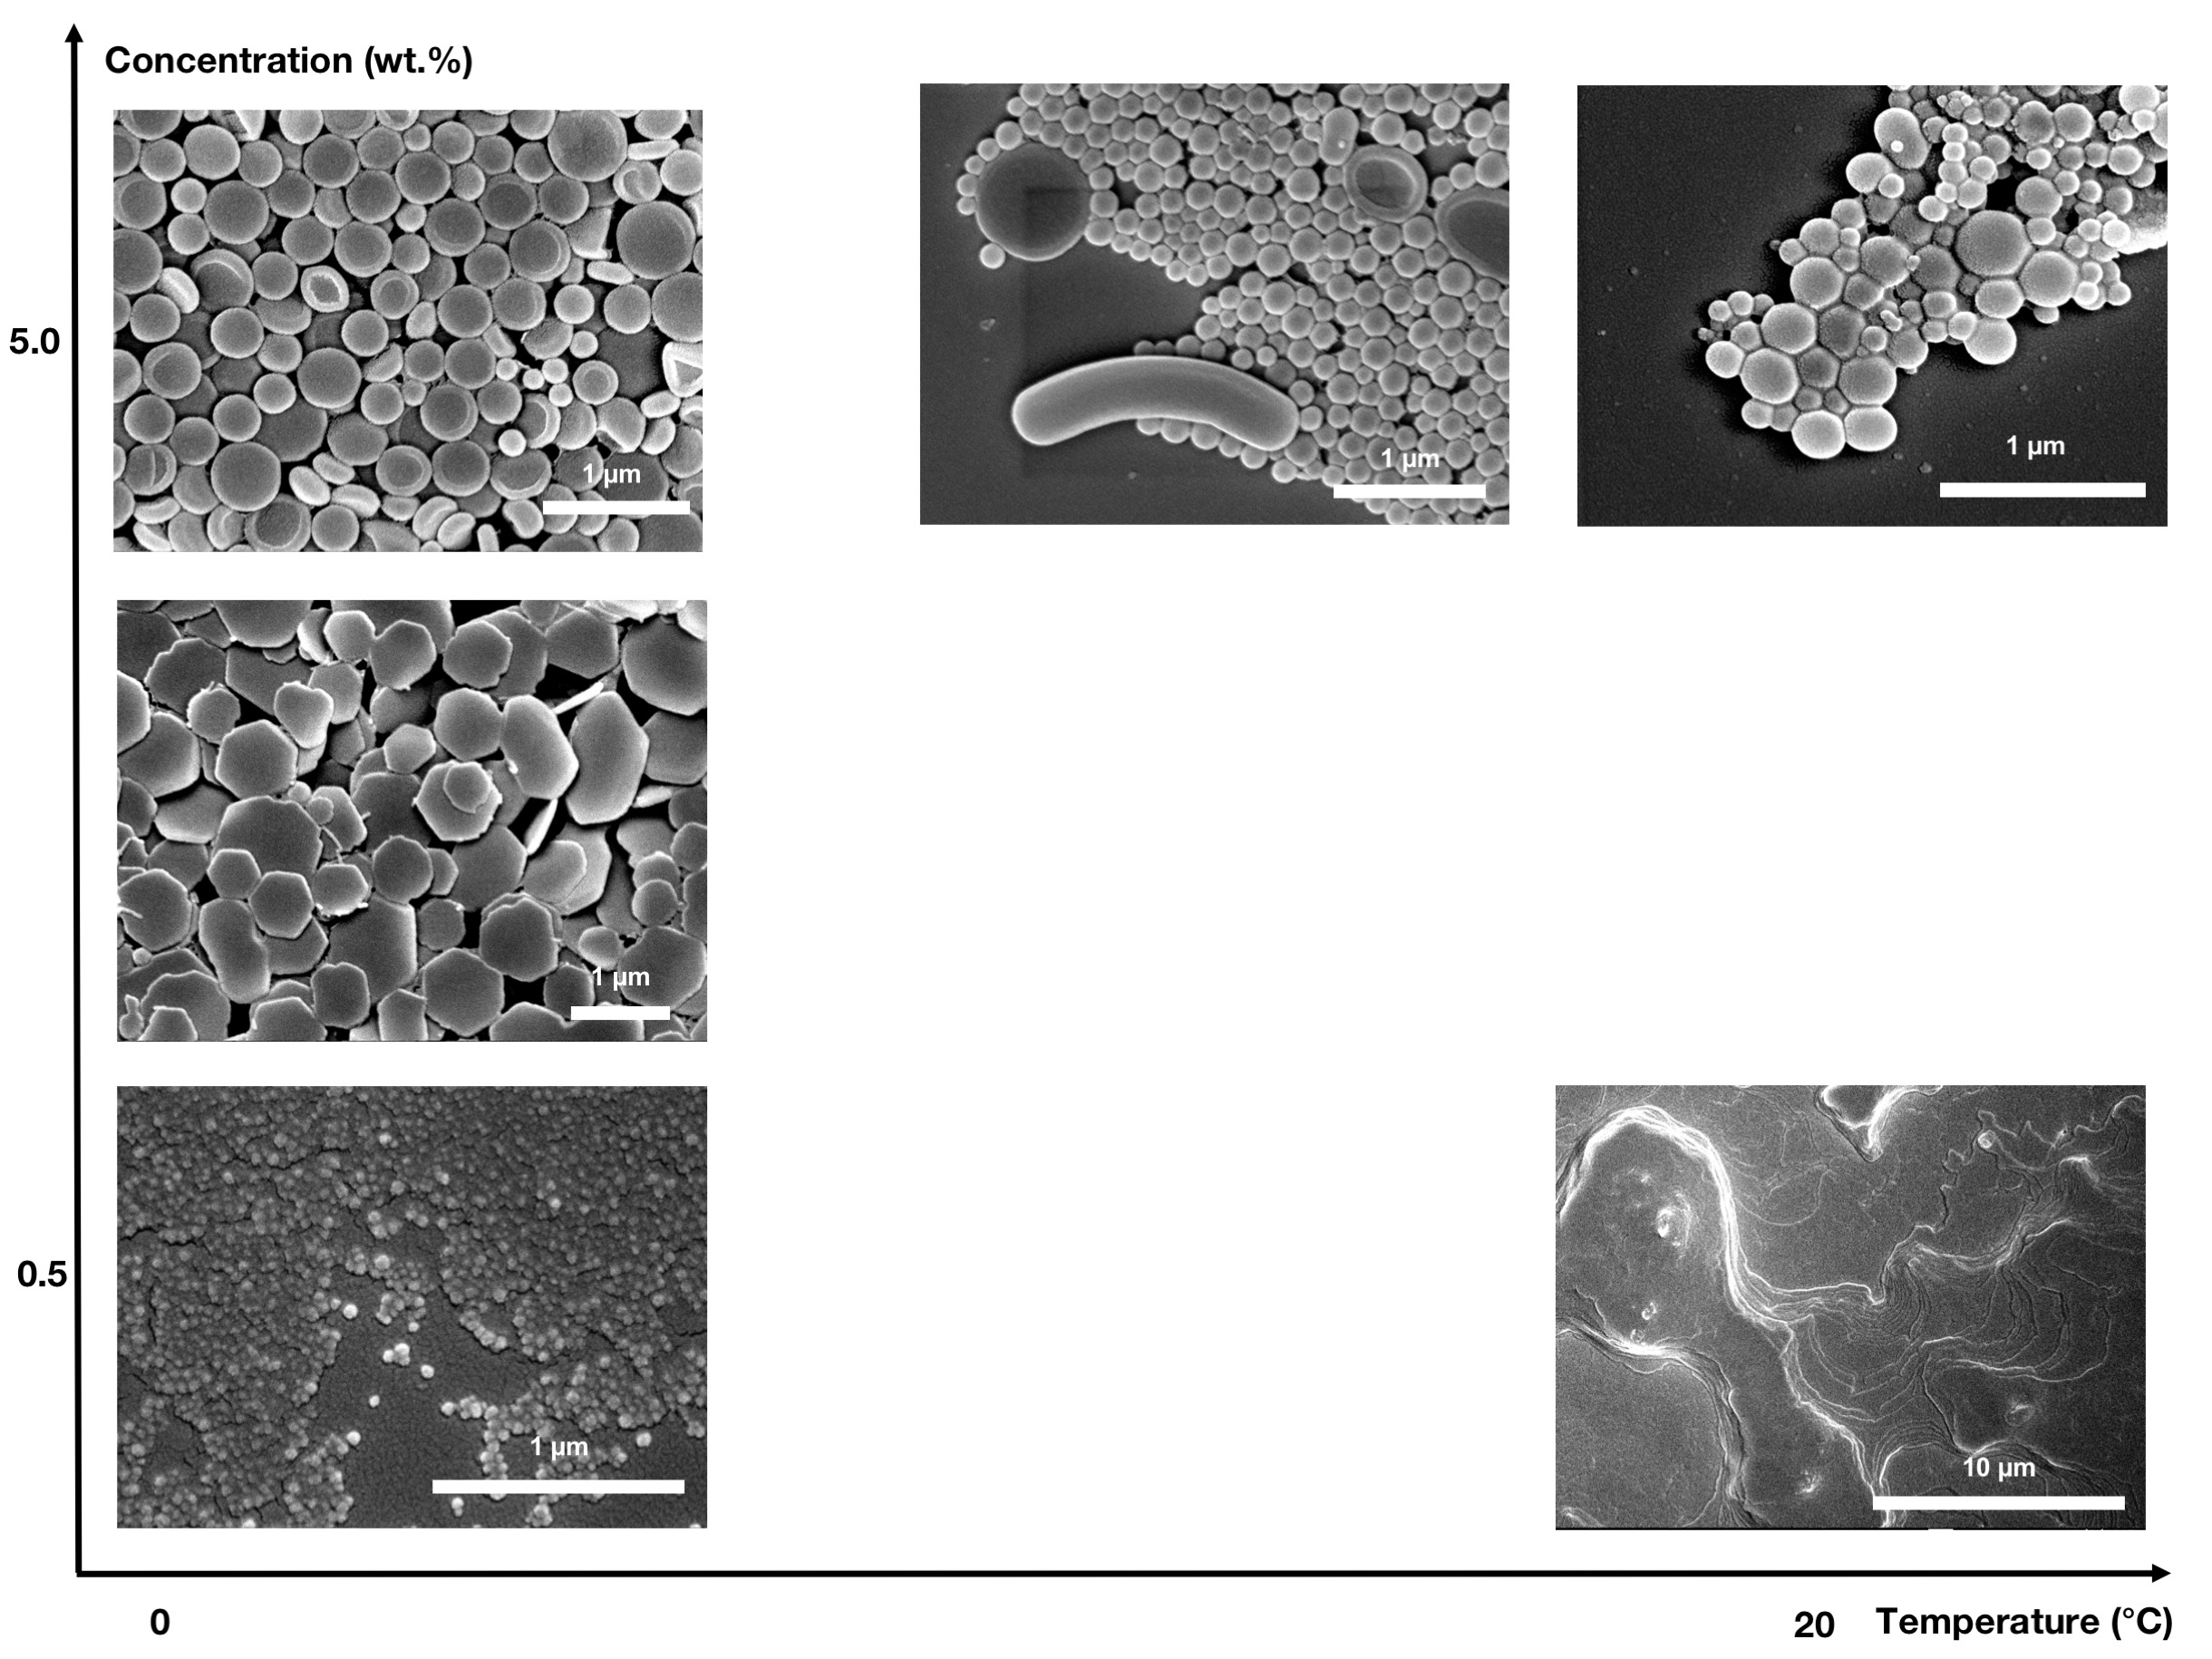
\includegraphics[width=\linewidth]{trends.jpg}
  		\caption{SEM micrographs highlighting various trends within the synthesis matrix.}
  	\end{figure}
	 
	 Through considering the ionic equilibria of the phosphate counterion, the hydrolysis state of the phosphate counterion is known to be pH-dependent by definition (Section 3.1). As it was previously established that the phase behaviour of \ce{DDA+} surfactants is affected by the hydrolysis state of the counterion \cite{liu2014}, we propose that solution pH is another dimension of control over the templating behaviour of \ce{DDAH_2PO_4} that can be investigated. This is a marked advantage over surfactant systems with monovalent counterions, as the pH of the solution can be modified without introducing spectator ions. A further parameter for exploration into the creation of new morphologies is doping quantities of different cations into the surfactant template solution. As mentioned previously, the addition of salts and electrolytes can affect changes in the self-assembly behaviour of surfactant microstructures \cite{thalberg1991}. We predict that introducing positively-charged electrolytes may disrupt hydrogen bonding and ion-dipole interactions in the solvation shell of the surfactant counterion, leading to changes in the self-assembled surfactant microstructures.
	
	Discovering a wide range of silica nanostructure morphologies poses exciting implications for their application in the creation of biomedical solutions such as artificial platelets. The effects of platelet geometry on their activation and action in wound repair have been well-studied \cite{sakurai2015,kita2011}. It has been found that silica nanoparticles have a positive effect on blood coagulation, with potential as a haemostatic agent for preventing blood loss after trauma \cite{gryshchuk2016}. We believe that further functionalization of geometrically specific silica platelets with coagulation factors and thrombin may prove to be a viable bioengineered solution for an active intervention in wound repair.
	
	\raggedbottom 
	\pagebreak
	\onecolumn
	\printbibliography
	
	\pagebreak
	
	\renewcommand{\thefigure}{S\arabic{figure}}

	\setcounter{figure}{0}
	
	\section*{Supplementary Information}

    \begin{thm}The expression of the fractional composition of various phosphate counteranions at different hydrolysis states as a function of hydronium ion concentration.
    \end{thm}


	\begin{proof} First, we consider the equilibrium expressions for the acidity dissociation constant $K_a$ values of each successive deprotonation of \ce{H_3PO_4}.

		\begin{equation*}
 		\ce{H3PO4(aq) + H2O(l) <=> H3O+(aq) + H2PO4^-(aq)}
 		\end{equation*}
 		\begin{equation*}
 		\ce{H2PO4^-(aq) + H2O(l) <=> H3O+(aq) + HPO4^{2-}(aq)}
 		\end{equation*}
 		\begin{equation*}
 		\ce{HPO4^{2-}(aq) + H2O(l) <=> H3O+(aq) + PO4^{3-}(aq)}
 		\end{equation*}
 		\begin{equation*}
 		K_{a1}=\frac{\ce{[H3O+][H2PO4^-]}}{\ce{[H3PO4]}} \qquad K_{a2}=\frac{\ce{[H3O+][HPO4^{2-}]}}{\ce{[H2PO4^-]}}
 		\qquad K_{a3}=\frac{\ce{[H3O+][PO4^{3-}]}}{\ce{[HPO4^{2-}]}}
 		\end{equation*}

 	Thereafter, we consider that the initial concentration of phosphoric acid in aqueous solution $P$, can be expressed as
 	the sum of the concentration of phosphoric acid in all its forms.

 		\begin{eqnarray}
 		\text{initial concentration } P & = & \ce{[H3PO4]}_\text{as prepared} \nonumber \\
 		& = & \ce{[H3PO4] + [H2PO4^-] + [HPO4^{2-}] + [PO4^{3-}]} \nonumber
 		\end{eqnarray}

 	We then manipulate the $K_a$ expressions such the concentrations of all species present can be expressed in terms of \ce{[H_3PO_4]} and \ce{[H3O+]}, along with the three acidity constants.

 	\begin{eqnarray}
 		\ce{[H2PO4^{-}]} & = & \frac{K_{a1}\ce{[H3PO4]}}{\ce{[H3O+]}} \nonumber \\
 		\ce{[HPO4^{2-}]} & = & \frac{K_{a1}K_{a2}\ce{[H3PO4]}}{\ce{[H3O+]}} \nonumber \\
 		\ce{[PO4^{3-}]} & = & \frac{K_{a1}K_{a2}K_{a3}\ce{[H3PO4]}}{\ce{[H3O+]}} \nonumber
 		\end{eqnarray}

 	The above results are then substituted into the expression for $P$, followed by factoring out the common \ce{[H_3PO_4]} term.

 	\begin{eqnarray}
 		P & = & \ce{[H_3PO_4]} + \frac{K_{a1}\ce{[H3PO4]}}{\ce{[H3O+]}} + \frac{K_{a1}K_{a2}\ce{[H3PO4]}}{\ce{[H3O+]}} + \frac{K_{a1}K_{a2}K_{a3}\ce{[H3PO4]}}{\ce{[H3O+]}}  \nonumber \\
 		& = & \Big\{ 1 + \frac{K_{a1}}{\ce{[H3O+]}} + \frac{K_{a1}K_{a2}}{\ce{[H3O+]^2}} + \frac{K_{a1}K_{a2}K_{a3}}{\ce{[H3O+]^3}} \Big\}\ce{[H3PO4]} \nonumber \\
 		& = & \frac{1}{\ce{[H3O+]^3}} \{ \ce{[H3O+]^3} + \ce{[H3O+]^2}K_{a1} + \ce{[H3O+]}K_{a1}K_{a2} + K_{a1}K_{a2}K_{a3}\}\ce{[H3PO4]} \nonumber
 		\end{eqnarray}


	Factoring out the $\frac{1}{\ce{[H3O+]^3}}$ term will make manipulation easier, as we will see in the next steps. Now we express each species fraction as a dissociation degree, as a function of $\ce{[H3O+]}$.

 	\begin{eqnarray}
 		\alpha_{\ce{H3PO4}} & = & \frac{\ce{[H3PO4]}}{P} \hspace{-10cm} \nonumber \\
 		& = & \frac{\ce{[H3PO4]}}{\frac{1}{\ce{[H3O+]^3}} \{ \ce{[H3O+]^3} + \ce{[H3O+]^2}K_{a1} + \ce{[H3O+]}K_{a1}K_{a2} + K_{a1}K_{a2}K_{a3}\}\ce{[H3PO4]}} \nonumber \\
 		& = & \frac{\ce{[H3O+]^3}}{\ce{[H3O+]^3} + \ce{[H3O+]^2}K_{a1} + \ce{[H3O+]}K_{a1}K_{a2} + K_{a1}K_{a2}K_{a3}}
 		\end{eqnarray}

 	\begin{eqnarray}
 		\alpha_{\ce{H2PO4^{-}}} & = & \frac{\ce{[H2PO4^{-}]}}{P} \hspace{-10cm} \nonumber  \\
 		& = & \frac{K_{a1}\ce{[H3PO4]}}{P\ce{[H3O+]}} \nonumber \\
 		& = & \frac{K_{a1}\ce{[H3PO4]}}{\frac{1}{\ce{[H3O+]^3}} \{ \ce{[H3O+]^3} + \ce{[H3O+]^2}K_{a1} + \ce{[H3O+]}K_{a1}K_{a2} + K_{a1}K_{a2}K_{a3}\}\ce{[H3PO4][H3O+]}} \nonumber \\
 		& = & \frac{K_{a1}\ce{[H3O+]^2}}{\ce{[H3O+]^3} + \ce{[H3O+]^2}K_{a1} + \ce{[H3O+]}K_{a1}K_{a2} + K_{a1}K_{a2}K_{a3}}
 		\end{eqnarray}

 	\begin{eqnarray}
 		\alpha_{\ce{HPO4^{2-}}} & = & \frac{\ce{[HPO4^{2-}]}}{P} \hspace{-10cm} \nonumber  \\
 		& = & \frac{K_{a1}K_{a2}\ce{[H3PO4]}}{P\ce{[H3O+]^2}} \nonumber \\
 		& = & \frac{K_{a1}K_{a2}\ce{[H3PO4]}}{\frac{1}{\ce{[H3O+]^3}} \{ \ce{[H3O+]^3} + \ce{[H3O+]^2}K_{a1} + \ce{[H3O+]}K_{a1}K_{a2} + K_{a1}K_{a2}K_{a3}\}\ce{[H3PO4][H3O+]^2}} \nonumber \\
 		& = & \frac{K_{a1}K_{a2}\ce{[H3O+]}}{\ce{[H3O+]^3} + \ce{[H3O+]^2}K_{a1} + \ce{[H3O+]}K_{a1}K_{a2} + K_{a1}K_{a2}K_{a3}}
 		\end{eqnarray}

 	\begin{eqnarray}
 		\alpha_{\ce{PO4^{3-}}} & = & \frac{\ce{[PO4^{3-}]}}{P} \hspace{-10cm} \nonumber  \\
 		& = & \frac{K_{a1}K_{a2}K_{a3}\ce{[H3PO4]}}{P\ce{[H3O+]^3}} \nonumber \\
 		& = & \frac{K_{a1}K_{a2}K_{a3}\ce{[H3PO4]}}{\frac{1}{\ce{[H3O+]^3}} \{ \ce{[H3O+]^3} + \ce{[H3O+]^2}K_{a1} + \ce{[H3O+]}K_{a1}K_{a2} + K_{a1}K_{a2}K_{a3}\}\ce{[H3PO4][H3O+]^3}} \nonumber \\
 		& = & \frac{K_{a1}K_{a2}K_{a3}}{\ce{[H3O+]^3} + \ce{[H3O+]^2}K_{a1} + \ce{[H3O+]}K_{a1}K_{a2} + K_{a1}K_{a2}K_{a3}}
 		\end{eqnarray}
	\\[2\baselineskip]
	The above fractions are then plotted against pH in Fig. S1.

 	%$begin{equation*}
 	%	H =  \ce{[H3O+]^3} + \ce{[H3O+]^2}K_{a1} + \ce{[H3O+]}K_{a1}K_{a2} + K_{a1}K_{a2}K_{a3}
 	%	\end{equation*}


	\end{proof}
	
	\pagebreak
	
	\begin{figure}[t!]
		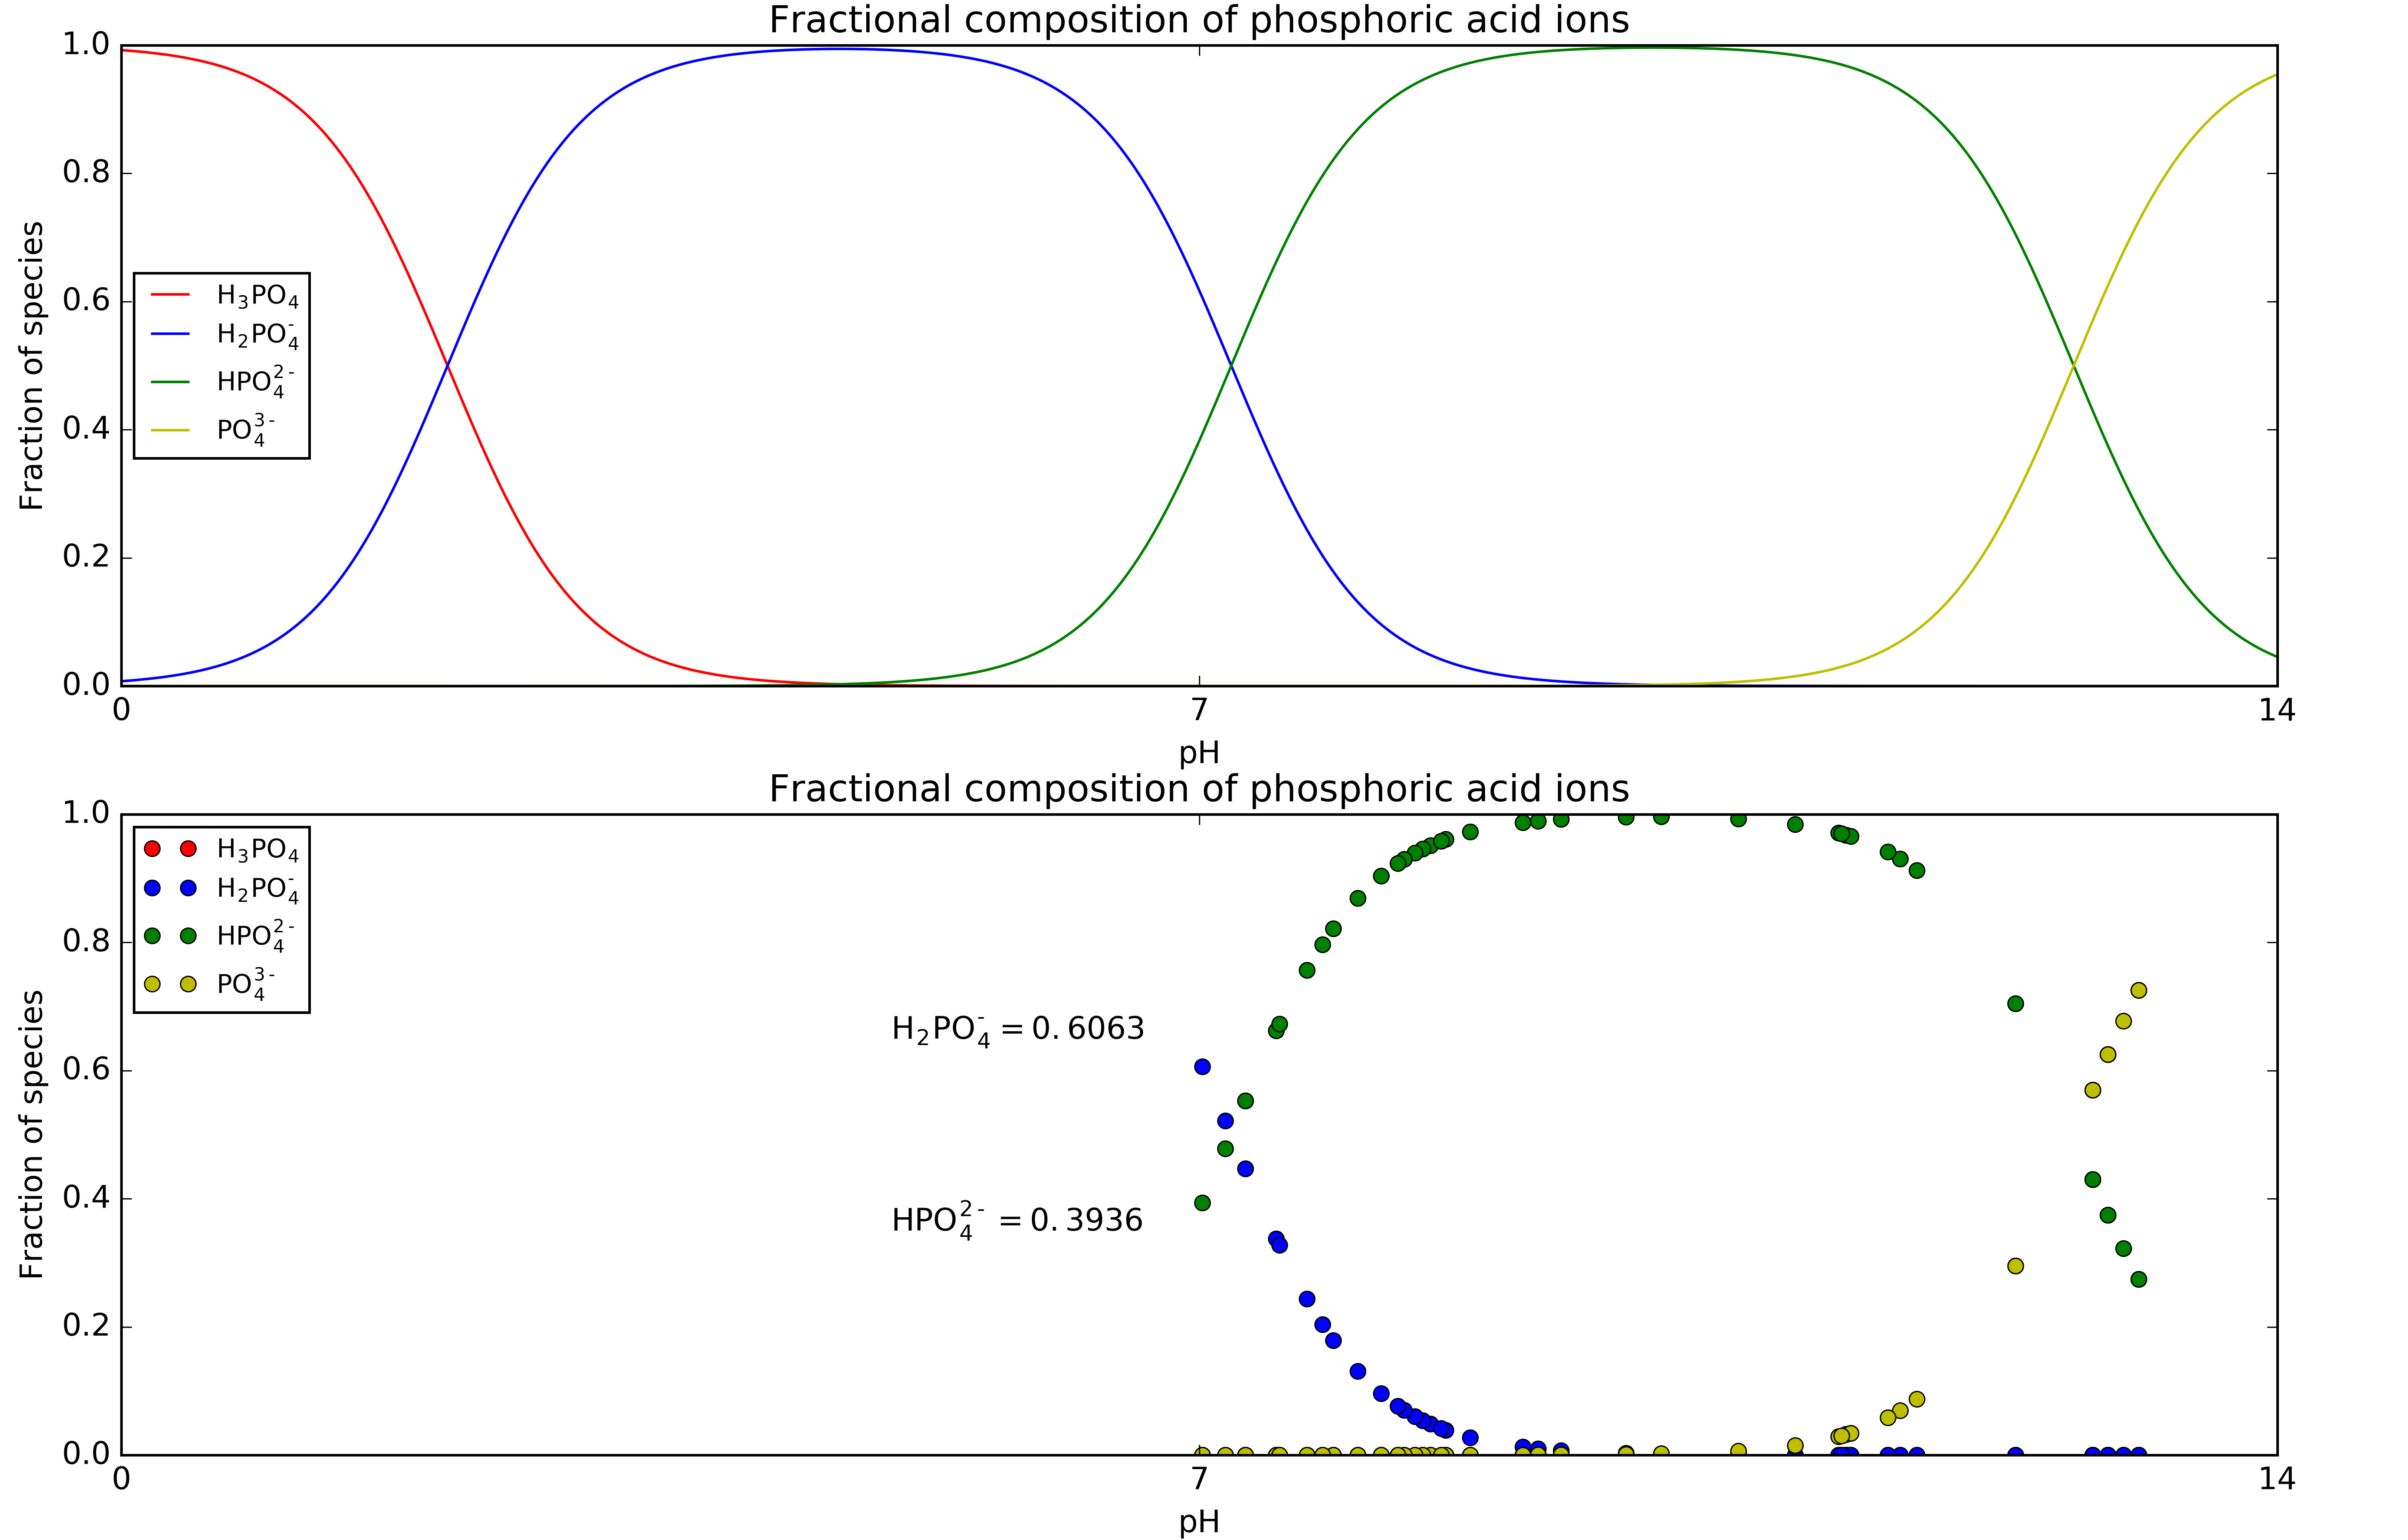
\includegraphics[width=\linewidth]{phosfraction.png}
  		\caption{Fractional composition of phosphoric acid ions for a given pH. Top: Theoretical range of speciation, Bottom: Range of speciation achieved in titration of phosphoric acid into DDAOH until an endpoint of pH 7.02.}
  	\end{figure}
	 
	\end{document}

